The main goal of this section is twofold. First, we show that the FE
discretization of the streamfunction formulation of the SQGE \eqref{sqge_psi_1}
with the Argyris element produces accurate numerical approximations. To this
end, we benchmark our numerical results against those in the published
literature \cite{Vallis06, Cascon, Myers}. The second goal is to show that the
numerical results follow the theoretical error estimates in
\autoref{thm:EnergyNorm} and \autoref{thm:Errors}, i.e., we compare the observed
rates of convergence to the theoretical rates of convergence developed in
\autoref{sec:SQGEErrors}.

Although the pure streamfunction formulation of the steady SQGE
\eqref{sqge_psi_1} is our main concern, we also test our Argyris FE
discretization on two simplified settings: \begin{inparaenum}[(i)] \item the
\emph{Linear Stommel} model; and \item \emph{Linear Stommel-Munk} model.
\end{inparaenum} The reason for using these two additional numerical tests is
that they are standard test problems in the geophysical fluid dynamics
literature (see, e.g., Chapter 13 in Vallis \cite{Vallis06} as well as the
reports of Myers \emph{et al.} \cite{Myers}, and Cascon \emph{et al.}
\cite{Cascon}). This allows us to benchmark our numerical results against
those in the published literature. Since both the Linear Stommel and the
Linear Stommel-Munk models lack the nonlinearity present in the SQGE
\eqref{sqge_psi_1}, the represent good stepping stones to verifying our FE
discretization.

The \emph{Linear Stommel-Munk} model (see p. 587 in \cite{Vallis06} and problem
2 in \cite{Cascon}) is given by
\begin{equation}
  \epsilon_s \Delta \psi - \epsilon_m \Delta^2 \psi + \frac{\partial \psi}{\partial x} = f,
  \label{eqn:Stommel-Munk}
\end{equation}
where $\epsilon_s \text{ and } \epsilon_m$ are the Stommel Number and Munk
Scale, respectively. The Stommel Number and Munk Scale are given by (Equation 10
in \cite{Myers})
\begin{equation*}
  \epsilon_m = \frac{A}{\beta L^3} \qquad \epsilon_s = \frac{\gamma}{\beta L}
\end{equation*}
where $A,\, \beta,\, L, \text{ and } \gamma$ are the eddy visosity, the
$\beta$-plane effect, characteristic length scale, and the bottom friction decay
rate, respectively. The model is supplemented with appropriate boundary
conditions, which will be described for each of the subsequent numerical tests.

We note that the Linear Stommel-Munk model \eqref{eqn:Stommel-Munk} is similar
in form to the SQGE \eqref{sqge_psi_1}. Indeed, both models contain the
biharmonic operator $\Delta^2 \psi$, the rotation term $\dfrac{\partial
\psi}{\partial x}$, and the forcing term $F$. The two main differences between
the two models are the following: First, the SQGE are nonlinear, since they
contain the Jacobian term $J(\psi,q)$; the Stommel-Munk model is linear, since
it doesn't contain the Jacobian term. The second difference is that the Linear
Stommel-Munk model contains a Laplacian term $\Delta \psi$, whereas the SQGE
does not.

We also note that the two models use different parameters: the Reynolds number
$Re$ and the Rossby number $Ro$ in \eqref{sqge_psi_1} and the Stommel number
$\epsilon_s$ and the Munk scale $\epsilon_m$ in the Linear Stommel-Munk model.
These two sets of parameters, however, are related by the following relations:
\begin{align}
  \epsilon_m &= Ro\, Re^{-1} \label{eqn:MunkScale}\\
  \epsilon_s &= Ro \frac{\gamma\, L}{U} \label{eqn:StommelNumber}\\
\end{align}
%\textcolor{red}{If $\gamma \sim T$ then $\epsilon = Ro$. However, I am unsure this is a valid
%assumption and so I am having trouble relating the Stommel Number to Reynolds and Rosby.}

The second simplified model used in our numerical investigation is the
\emph{Linear Stommel} model (Equation 14.22 in \cite{Vallis06} and Equation 11
in \cite{Myers})
\begin{equation}
  \epsilon_s \Delta \psi + \frac{\partial \psi}{\partial x} = f.
  \label{eqn:Stommel}
\end{equation}
We note that the Linear Stommel Model \eqref{eqn:Stommel} is just the Linear
Stommel-Munk model \eqref{eqn:Stommel-Munk} in which the biharmonic term is
dropped (i.e. $\epsilon_m=0$).

The rest of the subsection is organized as follows: In \autoref{sse:LSM} we
present results for the Linear Stommel model \eqref{eqn:Stommel}. In
\autoref{sse:SMM} we present results for the Linear Stommel-Munk model
\eqref{eqn:Stommel-Munk}. Finally, in \autoref{sse:SQGE} we present results for
the nonlinear SQGE \eqref{sqge_psi_1}.

\subsection{Linear Stommel Model} \label{sse:LSM} This subsection presents the
results for the FE discretization of the Linear Stommel model
\eqref{eqn:Stommel} by using the Argyris element. The computational domain is
$\Omega = [0,1]\times [0,1]$. For completeness, we present results for two
numerical tests. The first test, denoted by Test 1, corresponds to the exact
solution used by Vallis (Equation 14.38 in \cite{Vallis06}), while the second
test, denoted by Test 2, corresponds to the exact solution used by Myers
\emph{et al.} (Equations 15 and 16 in \cite{Myers}).

\tbf{Test 1a:} In this test, we choose the same setting as that used by Vallis
(Equation 14.38 in \cite{Vallis06}).  In particular, the forcing term and the
non-homogeneous Dirichlet boundary conditions are chosen to match those given by
the exact solution
\begin{equation}
  \psi(x,y) = (1-x-e^{-\nicefrac{x}{\epsilon_s}}) \sin \pi y
  \label{eqn:MyerExact}
\end{equation}
We choose the same Stommel number as that used by Vallis, i.e.
$\epsilon_s=0.04$. The exact solution \eqref{eqn:MyerExact} considered by Vallis
satisfies $\psi \to 0$ as $x \to 0$, but does not vanish at $x=1$. In our
numerical tests, we used a standard lifting procedure to treat these
non-homogeneous boundary conditions, i.e. for a problem of the form
\begin{align*}
  L \psi&=f \text{ on } \Omega\\
  \psi &=g \text{ on } \partial \Omega,
\end{align*}
we reformulate it to be
\begin{align*}
  L\tilde{\psi} &= \tilde{f} \text{ on } \Omega \\
  \tilde{\psi} &= 0 \text{ on } \partial \Omega
\end{align*}
where $L\tilde{\psi} = Lu - LS = f - g = \tilde{f}$ and the solution $\psi$ from
the original problem can then be found by $\psi(x,y) =\tilde{\psi}+S$. The
function $S(x,y)$ is assumed to have the form
\begin{equation*}
  S(x,y) = A(y) (1-x) + B(y) x
\end{equation*}
and satisfies the boundary conditions given by \eqref{eqn:MyersExact}. After
some simple algebra we see that
\begin{equation*}
  S(x,y) = -x e^{-x/\epsilon_s}\pi \sin(\pi y).
\end{equation*}
The function $\tilde{f}$ can be determined by applying the operator $L$
corresponding to the \emph{Linear Stommel} problem to $u - S$

Applying the finite element method to the \emph{Linear Stommel} problem with the
new modified $\tilde{f}$, corresponding to the exact solution given by Vallis,
and homogeneous boundary conditions using Argyris Finite Elements we get a
solution that matches the solution presented by Vallis, as can be seen in
\autoref{fig:StommelVallis}. Additionally, the table of errors
\autoref{tab:StommelErrorsVallis} shows the order of convergence appears to be
approaching the expected rates for $L^2, H^1, \text{ and } H^2$ norms.
\autoref{fig:StommelVallis} presents the streamlines of the approximate solution
obtained by using the Argyris Finite Element on a mesh with $h=\frac{1}{32}$ and
$9670$ DoFs. Comparing \autoref{fig:StommelVallis} with Figure $14.5$ in
\cite{Vallis06}, we notice that our approximation is close to his. Since the
exact solution is available, we can compute the errors in various norms.
\autoref{tab:StommelErrorsVallis} presents the errors $e_0,\, e_1, \text{ and }
e_2$ (i.e., the $L^2,\, H^1, \text{ and } H^2$ errors, respectively) for various
values of the mesh sizes, $h$ (the DoFs are also included).

\begin{table}%[H]
\begin{center}
%{\footnotesize
\begin{tabular}{|c|c|c|c|c|c|c|c|}%c|c|}
  \hline
  $h$ & $DoFs$ & $e_0$ & $L_2$ order & $e_1$ & $H^1$ order & $e_2$ & $H^2$ order \\[0.2em] % & $e_{\infty}$ & $L_{\infty}$ order \\
  \hline
  $\nicefrac{1}{2}$ & $70$ & $0.1148$ & $-$ & $1.81$ & $-$ & $83.67$ & $-$ \\[0.2em] % & $0.00681$ & $-$ \\
  $\nicefrac{1}{4}$ & $206$ & $0.01018$ & $3.495$ & $0.312$ & $2.537$ & $25.48$ & $1.716$ \\[0.2em] % & $0.007801$ & $-0.1961$ \\
  $\nicefrac{1}{8}$ & $694$ & $0.0004461$ & $4.512$ & $0.02585$ & $3.593$ & $3.902$ & $2.707$ \\[0.2em] % & $0.0004681$ & $4.059$ \\
  $\nicefrac{1}{16}$ & $2534$ & $1.09\times 19^{-5}$ & $5.355$ & $0.001215$ & $4.412$ & $0.3494$ & $3.481$ \\[0.2em] % & $1.732\times 19^{-5}$ & $4.756$ \\
  $\nicefrac{1}{32}$ & $9670$ & $1.972\times 19^{-7}$ & $5.788$ & $4.349\times 19^{-5}$ & $4.804$ & $0.02335$ & $3.903$ \\[0.2em] % & $5.396\times 19^{-7}$ & $5.005$ \\
  \hline
\end{tabular}
%}
\end{center}
\caption{Errors and Rate of Convergence for the Linear Stommel Model \eqref{eqn:Stommel}, Test 1 \cite{Vallis06}}
\label{tab:StommelErrorsVallis}
\end{table}

\begin{figure}%[H]
  \begin{center}
    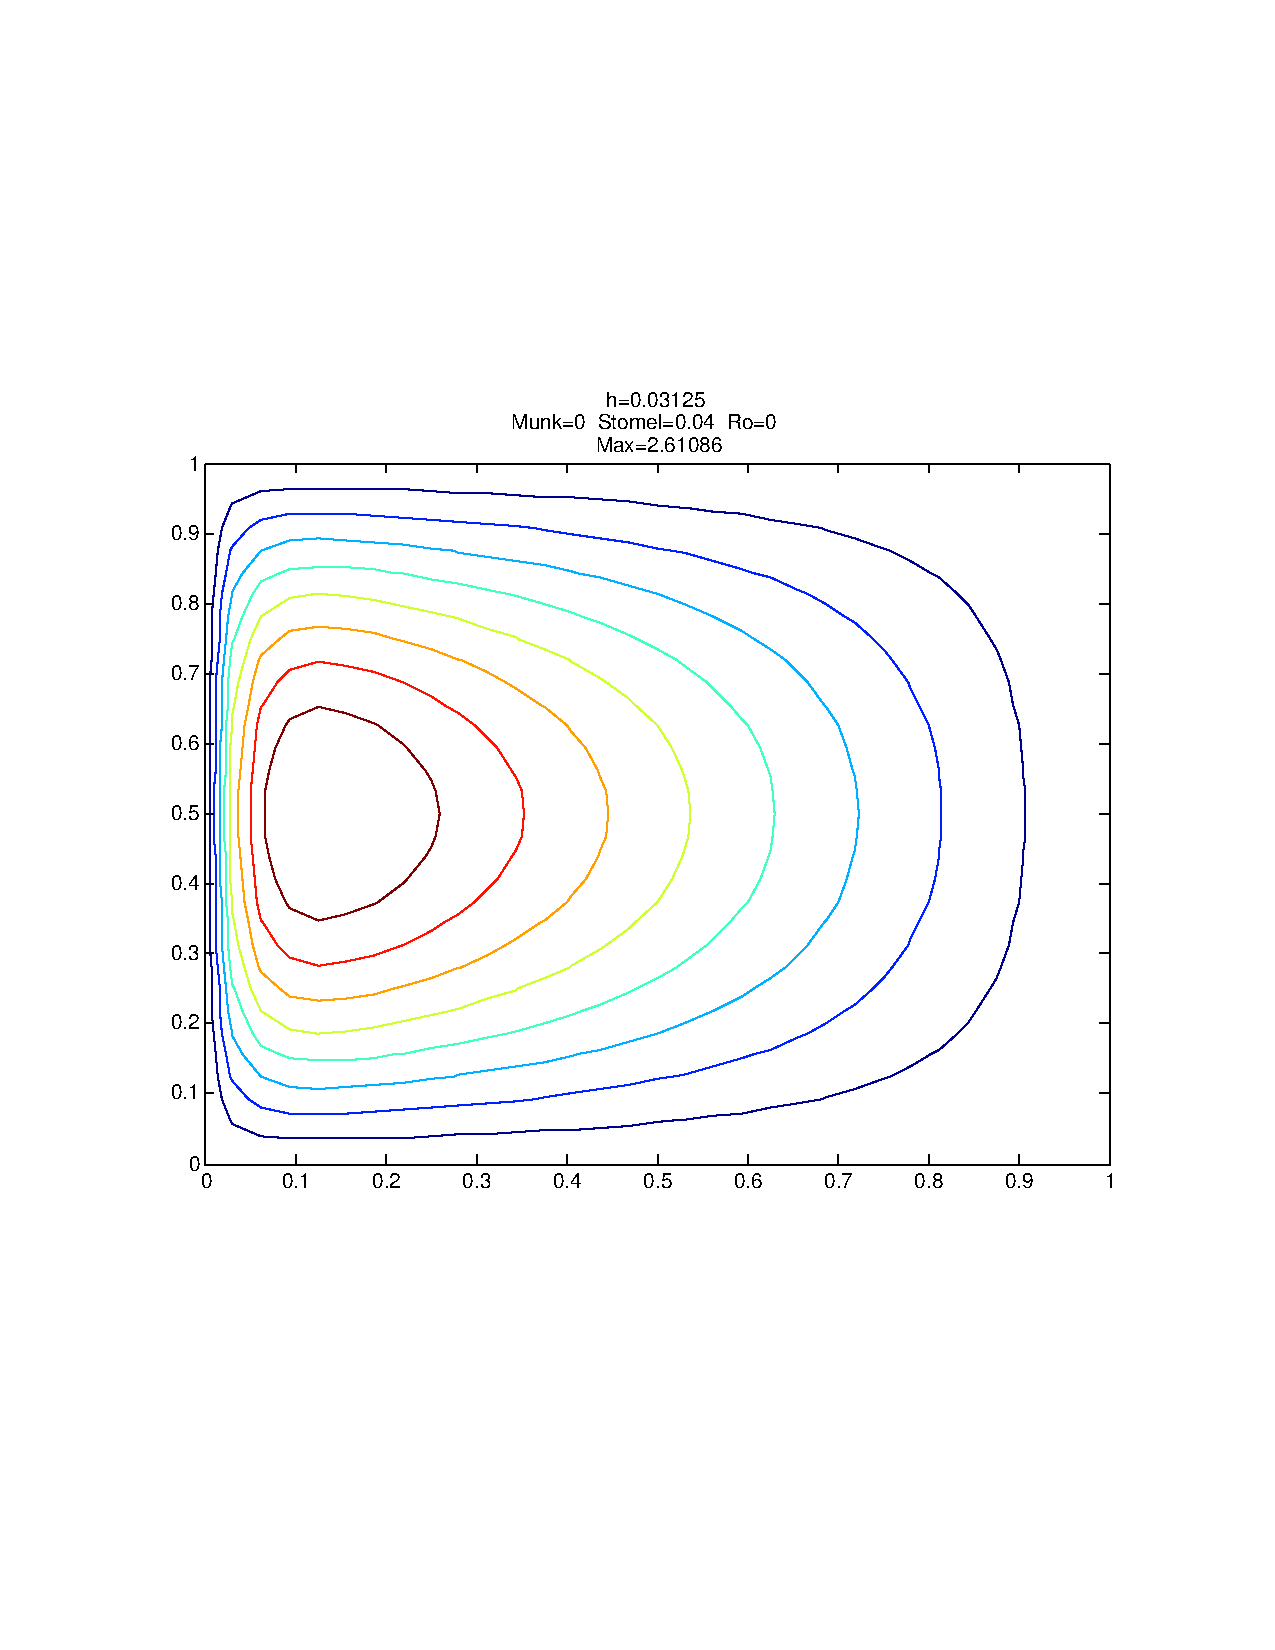
\includegraphics[trim=0 200 20 220, clip=true, scale=0.5]{LinearStommelVallis.pdf}
    \caption{Linear Stommel Model \eqref{eqn:Stommel}, Test 1a \cite{Vallis06}: Streamlines of the approximation,
    $\psi^h$, $h=\frac{1}{32}$, and $9670$ DoFs.}
    \label{fig:StommelVallis}
  \end{center}
\end{figure}
We note that the errors in \autoref{tab:StommelErrorsVallis} follow the
theoretical rates of convergence predicted by the estimates \eqref{eqn:H2Error}
- \eqref{eqn:L2Error} in \autoref{thm:Errors}. The orders of convergence in
\autoref{tab:StommelErrorsVallis} are close to the theoretical ones for the fine
meshes, but not as close for the coarse meshes. We think that the inaccuracies
on the coarse meshes are due to their inability to capture the thin boundary
layer on the left-hand side (i.e., at $x=0$). The finer the mesh gets, the
better this boundary layer is captured and the better the numerical accuracy
becomes.

\tbf{Test 1b:}
In the Second part of Test 1, we verify the hypothesis above, that is, whether
the degrading accuracy of the approximation is indeed due to the thin western
boundary layer. To this end, we change the Stommel number in Test 1a to be
$\epsilon_s=1$, which will result in a much thicker western boundary layer. We
then run the same numerical test as before, but with the new Stommel number. As
can be seen in \autoref{tab:StommelErrorsVallise1}, the rates of convergence are
the expected theoretical orders of convergence. This shows that the reason for
the inaccuracies in \autoref{tab:StommelErrorsVallis} were indeed due to the
thin western boundary layer.

\begin{table}%[H]
\begin{center}
%{\scriptsize
\begin{tabular}{|c|c|c|c|c|c|c|c|}%c|c|}
  \hline
  $h$ & $DoFs$ & $e_0$ & $L_2$ order & $e_1$ & $H^1$ order & $e_2$ & $H^2$ order \\[0.2em] % & $e_{\infty}$ & $L_{\infty}$ order \\
  \hline
  $\nicefrac{1}{2}$ & $70$ & $1.689\times 10^{-5}$ & $-$ & $0.0003434$ & $-$ & $0.008721$ & $-$ \\[0.2em] % & $4.306\times 10^{-6}$ & $-$ \\
  $\nicefrac{1}{4}$ & $206$ & $3.722\times 10^{-7}$ & $5.504$ & $1.341\times 10^{-5}$ & $4.678$ & $0.0005616$ & $3.957$ \\[0.2em] % & $5.542\times 10^{-7}$ & $2.958$ \\
  $\nicefrac{1}{8}$ & $694$ & $4.891\times 10^{-9}$ & $6.25$ & $3.757\times 10^{-7}$ & $5.158$ & $3.25\times 10^{-5}$ & $4.111$ \\[0.2em] % & $9.043\times 10^{-9}$ & $5.937$ \\
  $\nicefrac{1}{16}$ & $2534$ & $7.079\times 10^{-11}$ & $6.111$ & $1.117\times 10^{-8}$ & $5.071$ & $1.964\times 10^{-6}$ & $4.049$ \\[0.2em] % & $1.355\times 10^{-10}$ & $6.06$ \\
  $\nicefrac{1}{32}$ & $9670$ & $1.08\times 10^{-12}$ & $6.035$ & $3.437\times 10^{-10}$ & $5.023$ & $1.213\times 10^{-7}$ & $4.018$ \\[0.2em] % & $2.169\times 10^{-12}$ & $5.965$ \\
  \hline
\end{tabular}
%}
\end{center}
\caption{Errors and Rate of Convergence for the Linear Stommel Model \eqref{eqn:Stommel}, Test 1b \cite{Vallis06}}
\label{tab:StommelErrorsVallise1}
\end{table}

\begin{figure}%[H]
  \begin{center}
    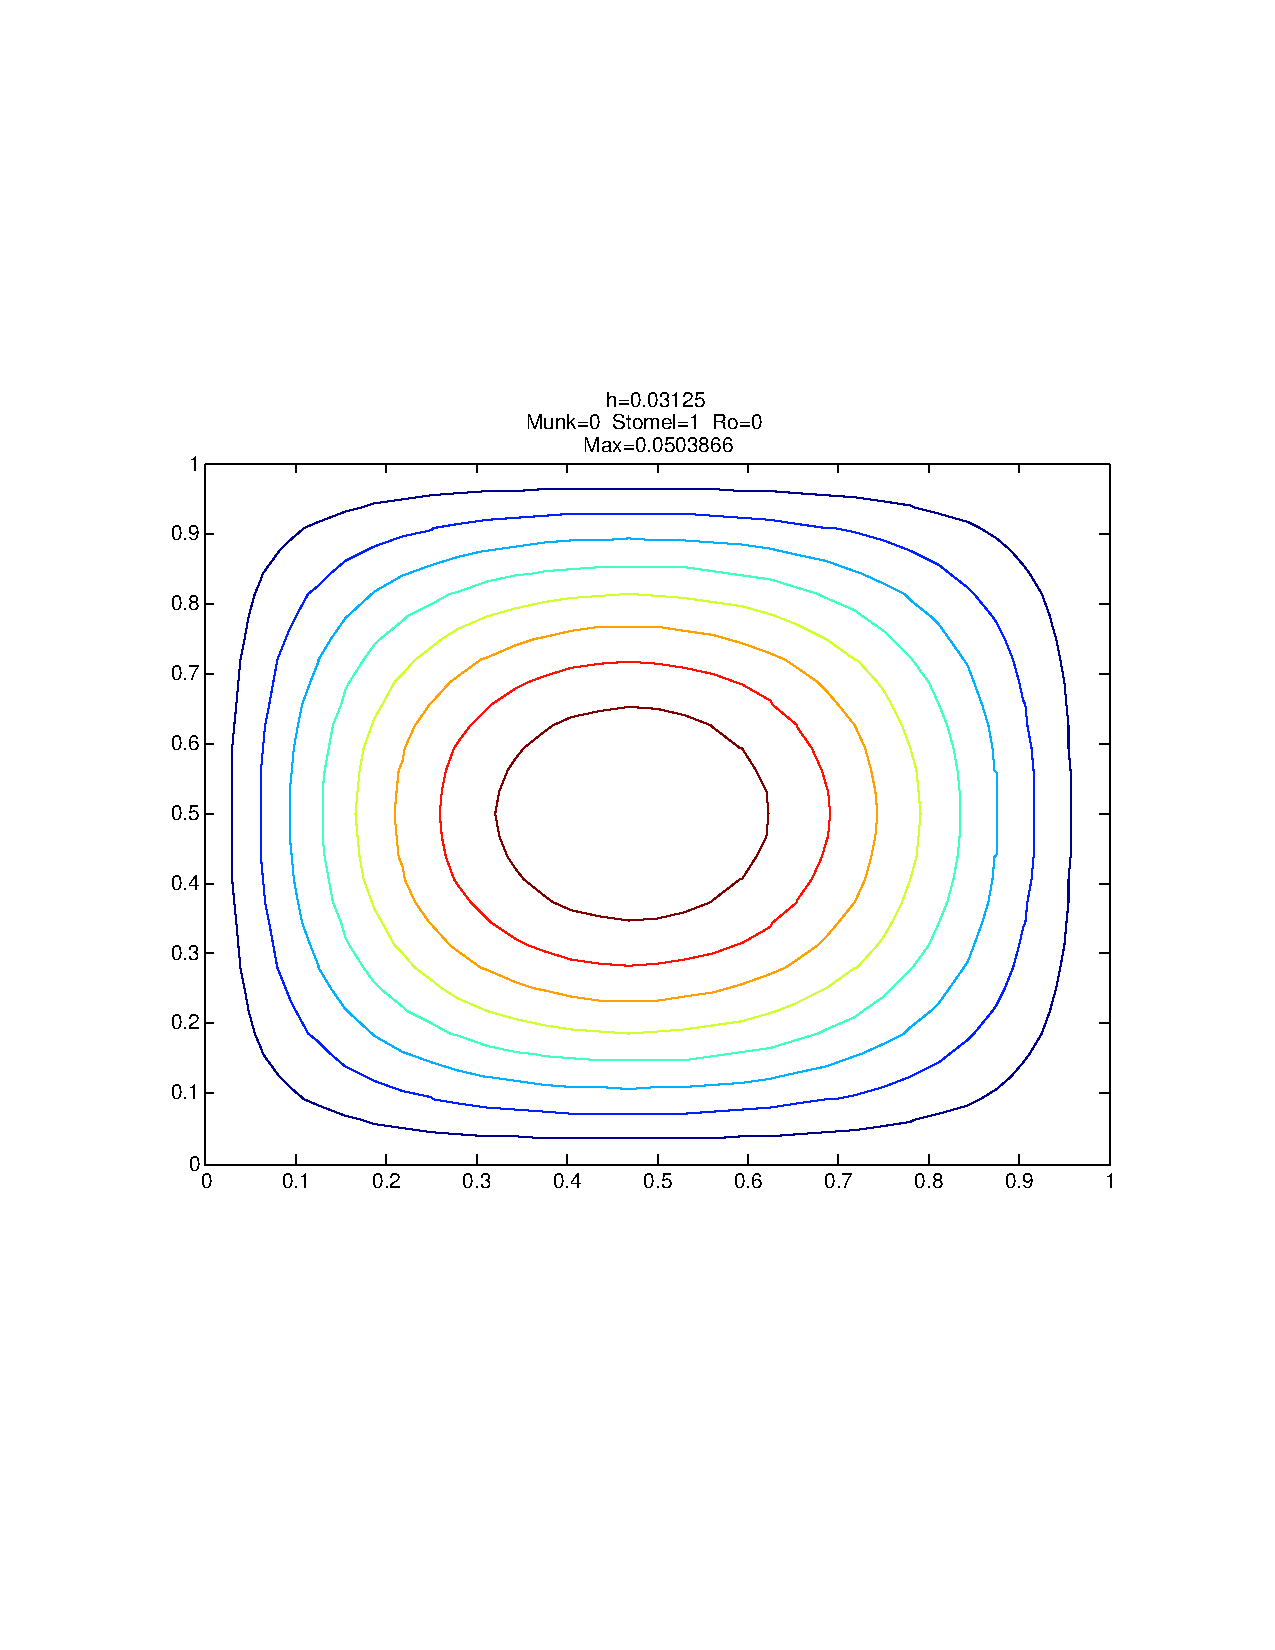
\includegraphics[trim=0 200 20 220, clip=true, scale=0.5]{StommelVallise1.pdf}
    \caption{Linear Stommel Model \eqref{eqn:Stommel}, Test 1b \cite{Vallis06}: Streamlines of the approximation,
    $\psi^h$, $h=\frac{1}{32}$, and $9670$ DoFs with $\epsilon_s=1$.}
    \label{fig:StommelVallise1}
  \end{center}
\end{figure}

\tbf{Test 2:}
For our second test we use the exact solution given by Myers (Equations 15 and
16 in \cite{Myers}), i.e.
{\footnotesize
\begin{equation}
  \psi(x,y) =\frac{\sin(\pi y)}{\pi(1+4\pi^2\epsilon_s^2)}\left\{2\pi\epsilon_s\sin(\pi x)+cos(\pi x)+\frac{1}{e^{R_1}-e^{R_2}}\left[(1+e^{R_2})e^{R_1x}-(1+e^{R_1})e^{R_2x}\right]\right\},
  \label{eqn:MyersExact}
\end{equation}
}
where $R_1\text{ and } R_2$ are the positive and negative roots, respectively,
of
\begin{equation*}
  R = \frac{-1\pm\sqrt{1+4\pi^2 \epsilon_s^2}}{2\epsilon_s}.
\end{equation*}
The forcing term and the homogeneous Dirichlet boundary conditions are chosen to
match those given by the exact solution \eqref{eqn:MyersExact}. We choose the
same Stommel number as that used by Myers, i.e. $\epsilon_s=0.05$.

\autoref{fig:StommelMyers} presents the streamlines of the approximate solution
obtained by using the Argyris Finite Element on a mesh with $h=\frac{1}{32}$ and
$9670$ DoFs. Comparing \autoref{fig:StommelMyers} with Figure $2$ in
\cite{Myers}, we notice that our approximation is close to that in \cite{Myers}.
Since the exact solution is available, we can compute the errors in various
norms. \autoref{tab:StommelErrorsMyers} presents the errors $e_0,\, e_1, \text{
and } e_2$ (i.e., the $L^2,\, H^1, \text{ and } H^2$ errors, respectively) for
various values of the mesh sizes, $h$.

\begin{table}%[H]
\begin{center}
%{\footnotesize
\begin{tabular}{|c|c|c|c|c|c|c|c|}%c|c|}
  \hline
  $h$ & $DoFs$ & $e_0$ & $L_2$ order & $e_1$ & $H^1$ order & $e_2$ & $H^2$ order \\[0.2em] % & $e_{\infty}$ & $L_{\infty}$ order \\
  \hline
  $\nicefrac{1}{2}$ & $70$ & $0.005645$ & $-$ & $0.1451$ & $-$ & $6.602$ & $-$ \\[0.2em] % & $0.0008815$ & $-$ \\
  $\nicefrac{1}{4}$ & $206$ & $0.0004276$ & $3.723$ & $0.02081$ & $2.801$ & $1.632$ & $2.016$ \\[0.2em] % & $0.0003139$ & $1.49$ \\
  $\nicefrac{1}{8}$ & $694$ & $1.46\times 10^{-5}$ & $4.872$ & $0.001408$ & $3.886$ & $0.2066$ & $2.982$ \\[0.2em] % & $2.15\times 10^{-5}$ & $3.868$ \\
  $\nicefrac{1}{16}$ & $2534$ & $2.954\times 10^{-7}$ & $5.627$ & $5.829\times 10^{-5}$ & $4.594$ & $0.0165$ & $3.646$ \\[0.2em] % & $7.097\times 10^{-7}$ & $4.921$ \\
  $\nicefrac{1}{32}$ & $9670$ & $4.968\times 10^{-9}$ & $5.894$ & $1.998\times 10^{-6}$ & $4.867$ & $0.001069$ & $3.948$ \\[0.2em] % & $2.054\times 10^{-8}$ & $5.111$ \\
  \hline
\end{tabular}
%}
\end{center}
\caption{Errors and Rate of Convergence for the Linear Stommel Model \eqref{eqn:Stommel}, Test 2 \cite{Myers}}
\label{tab:StommelErrorsMyers}
\end{table}

\begin{figure}%[H]
  \begin{center}
    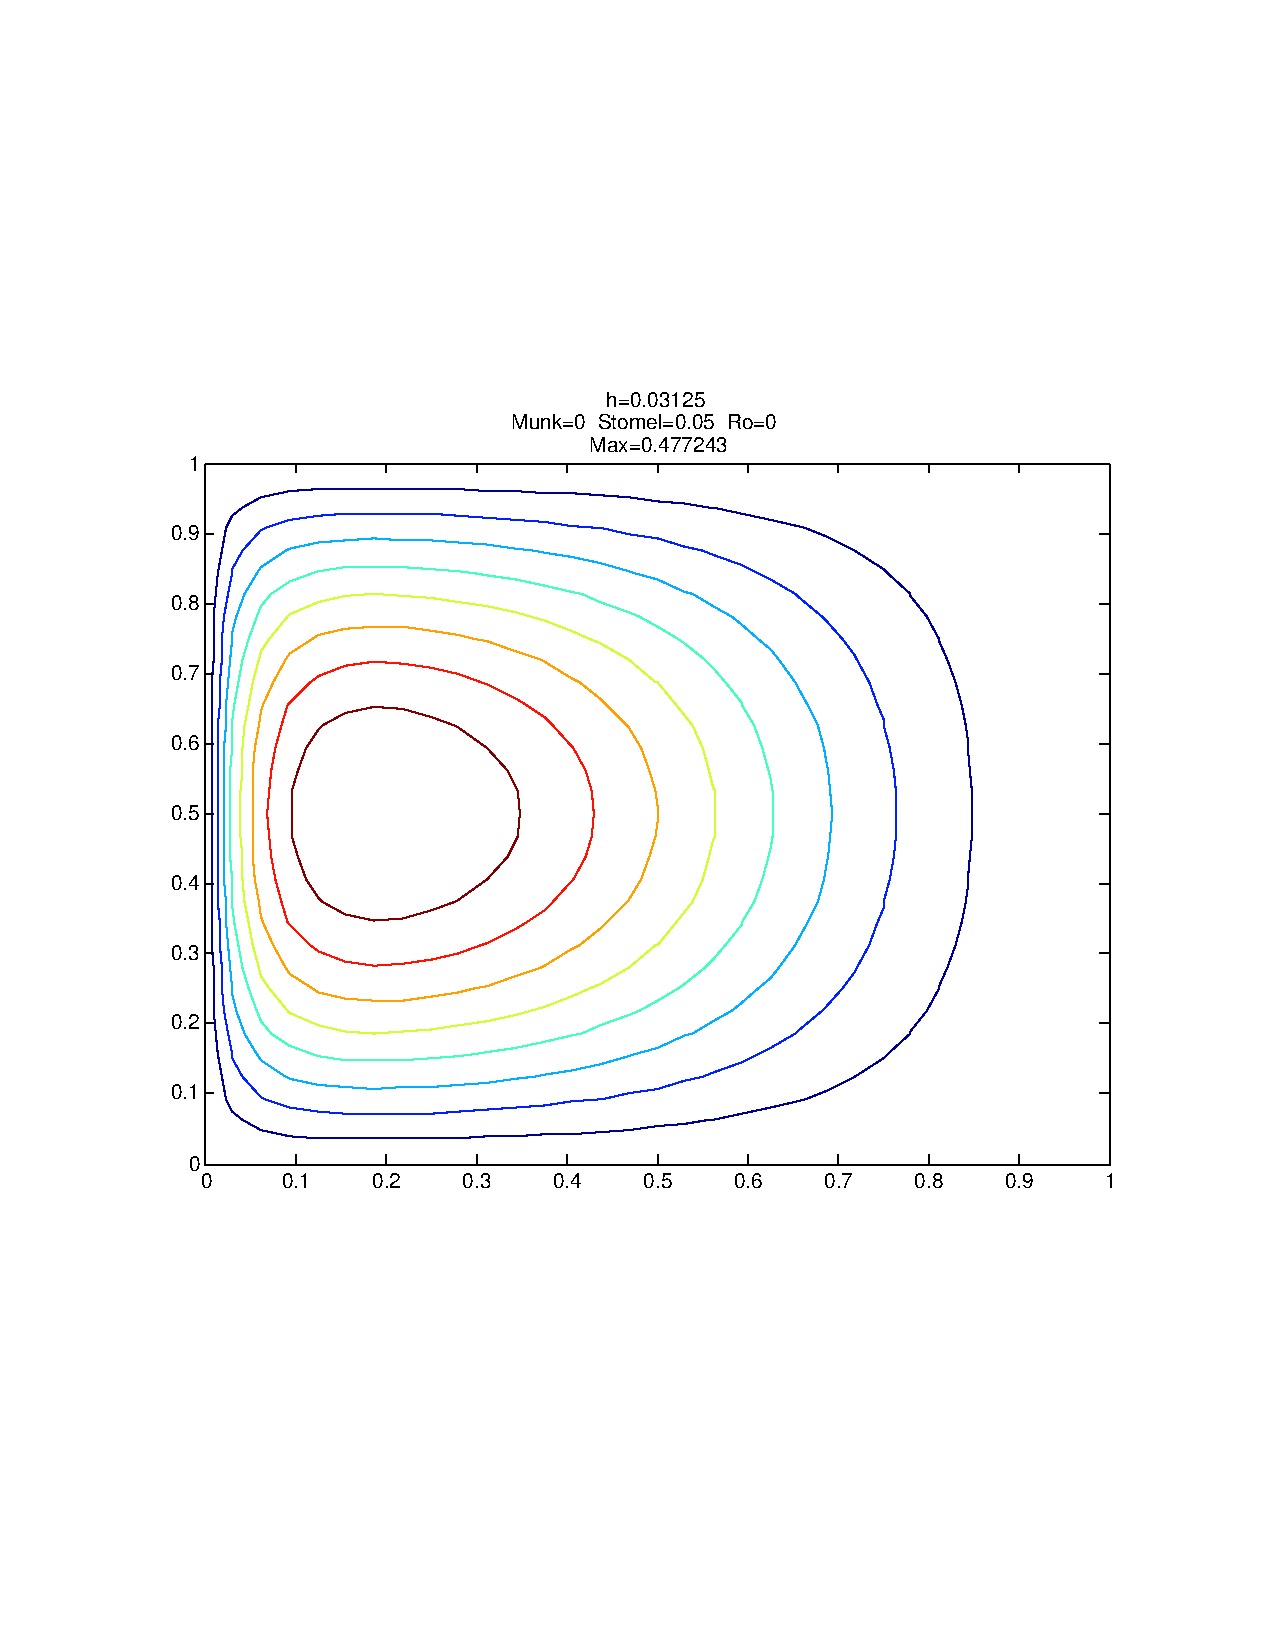
\includegraphics[trim=0 200 20 220, clip=true, scale=0.5]{LinearStommelMyers.pdf}
    \caption{Linear Stommel Model \eqref{eqn:Stommel}, Test 2 \cite{Myers}: Streamlines of the approximation,
    $\psi^h$, $h=\frac{1}{32}$, and $9670$ DoFs.}
    \label{fig:StommelMyers}
  \end{center}
\end{figure}

We note that the errors in \autoref{tab:StommelErrorsMyers} follow the
theoretical rates of convergence predicted by the estimates \eqref{eqn:H2Error}
- \eqref{eqn:L2Error} in \autoref{thm:Errors}. Again, we see that the orders of
convergence in \autoref{tab:StommelErrorsMyers} are close to the theoretical
ones for the fine meshes, but not as close for the coarse meshes. We attribute
this to the inaccuracies at the thin boundary layer on the left-hand side (i.e.,
at $x=0$). The finer the mesh gets, the better this boundary layer is captured
and the better the numerical accuracy becomes.

\subsection{Linear Stommel-Munk Model}\label{sse:SMM}
This subsection presents results for the FE discretization of the Linear
Stommel-Munk model \eqref{eqn:Stommel-Munk} by using the Argyris element. Our
computational setting is the same as taht used by Cascon \emph{et al.}
\cite{Cascon}: The computational domain is $\Omega = [0,3]\times[0,1]$, the Munk
scale is $\epsilon_m=6\times 10^{-5}$, the Stommel number is $\epsilon_s=0.05$,
and the boundary conditions are
\begin{equation} \label{eqn:SMProb}
  \psi = \frac{\partial \psi}{\partial \mathbf{n}}=0 \quad \text{ on } \partial\Omega
\end{equation}
For completeness, we present results for two numerical tests, denoted by Test 3
and Test 4, both corresponding to Test 1 and Test 2 in \cite{Cascon},
respectively.

\tbf{Test 3:}
For our third test we use the exact solution given by Test 1 in \cite{Cascon},
i.e.
\begin{equation}
  \psi(x,y) = \sin^2 \frac{\pi x}{3} \sin^2 \pi y.
  \label{eqn:CasconExact1}
\end{equation}
The forcing term is chosen to match that given by the exact solution
\eqref{eqn:CasconExact1}.

For this third test we take $F$ corresponding to applying the linear operator
$L$ associated with the \emph{Linear Stommel-Munk} model to the exact solution
\eqref{eqn:CasconExact1}.

\autoref{fig:StommelMunkSin} presents the streamlines of the approximate
solution obtained by using the Argyris Finite Element on a mesh with
$h=\frac{1}{32}$ and $28550$ DoFs. Comparing \autoref{fig:StommelMunkSin} with
Figure $7$ in \cite{Myers}, we notice that our approximation is close to that in
\cite{Myers}. Since the exact solution is available, we can compute the errors
in various norms. \autoref{tab:SMsinErrors} presents the errors $e_0,\, e_1,
\text{ and } e_2$ (i.e., the $L^2,\, H^1, \text{ and } H^2$ errors,
respectively) for various values of the mesh sizes, $h$.

\begin{table}%[H]
\begin{center}
%{\scriptsize
\begin{tabular}{|c|c|c|c|c|c|c|c|}%c|c|}
  \hline
  $h$ & $DoFs$ & $e_0$ & $L_2$ order & $e_1$ & $H^1$ order & $e_2$ & $H^2$ order \\[0.2em] % & $e_{\infty}$ & $L_{\infty}$ order \\
  \hline
  $\nicefrac{1}{2}$ & $170$ & $0.00299$ & $-$ & $0.04084$ & $-$ & $0.7624$ & $-$ \\[0.2em] % & $0.003423$ & $-$ \\
  $\nicefrac{1}{4}$ & $550$ & $3.217\times 10^{-5}$ & $6.539$ & $0.001031$ & $5.308$ & $0.04078$ & $4.225$ \\[0.2em] % & $1.885\times 10^{-5}$ & $7.505$ \\
  $\nicefrac{1}{8}$ & $1958$ & $3.437\times 10^{-7}$ & $6.548$ & $2.491\times 10^{-5}$ & $5.371$ & $0.002253$ & $4.178$ \\[0.2em] % & $2.371\times 10^{-7}$ & $6.313$ \\
  $\nicefrac{1}{16}$ & $7366$ & $4.571\times 10^{-9}$ & $6.232$ & $7.026\times 10^{-7}$ & $5.148$ & $0.0001344$ & $4.067$ \\[0.2em] % & $4.296\times 10^{-9}$ & $5.786$ \\
  $\nicefrac{1}{32}$ & $28550$ & $6.704\times 10^{-11}$ & $6.091$ & $2.113\times 10^{-8}$ & $5.056$ & $8.26\times 10^{-6}$ & $4.024$ \\[0.2em] % & $6.86\times 10^{-11}$ & $5.969$ \\
 \hline
\end{tabular}
%}
\end{center}
\caption{Errors and Rate of Convergence for the Linear Stommel-Munk Model \eqref{eqn:SMProb}, Test 3 \cite{Cascon}}
\label{tab:SMsinErrors}
\end{table}

\begin{figure}%[H]
  \begin{center}
    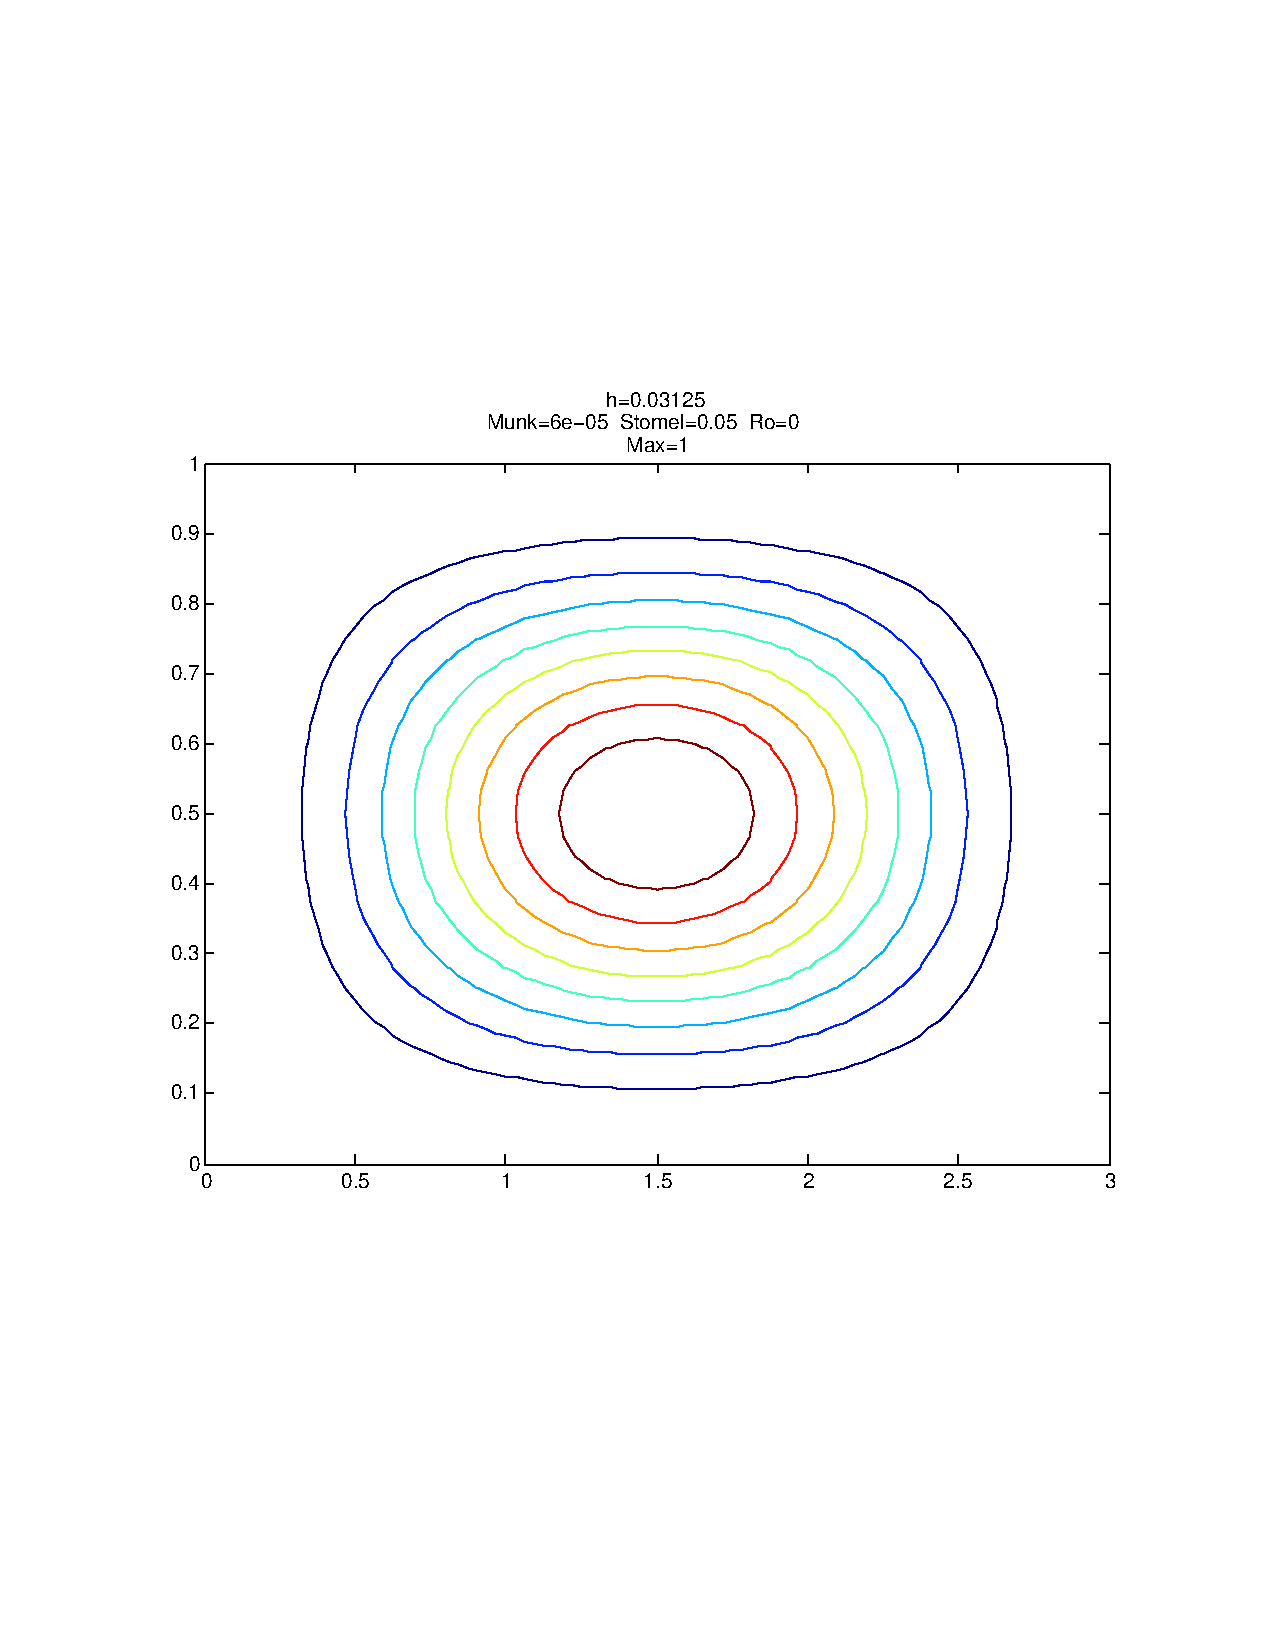
\includegraphics[trim=0 200 20 220, clip=true, scale=0.5]{StommelMunk1.pdf}
    \caption{Linear Stommel-Munk Model \eqref{eqn:SMProb}, Test 3 \cite{Cascon}: Streamlines of the approximation,
    $\psi^h$, on a mesh size, $h=\frac{1}{32}$, and $28550$ DoFs.}
    \label{fig:StommelMunkSin}
  \end{center}
\end{figure}

We note that the errors in \autoref{tab:SMsinErrors} follow the theoretical
rates of convergence predicted by the estimates \eqref{eqn:H2Error} -
\eqref{eqn:L2Error} in \autoref{thm:Errors}.  This time, we see that the orders
of convergence in \autoref{tab:SMsinErrors} are close to the theoretical ones
for the fine meshes, but are higher than expected for the for the coarse meshes.
We attribute this to the fact that the exact solution \eqref{eqn:CasconExact1}
does not display any boundary layers that could be challenging to capture by the
Argyris element on a coarse mesh.

\tbf{Test 4:}
For our fourth test we use the exact solution given by Test 2 in \cite{Cascon},
i.e.
{\small
\begin{equation}
  \psi(x,y) = \left[\left(1 - \frac{x}{3}\right)\left(1-e^{-20x}\right) \sin \pi y\right]^2.
  \label{eqn:CasconExact2}
\end{equation}
}
Again we take the forcing term $F$ corresponding the exact solution
\eqref{eqn:CasconExact2}.

\autoref{fig:SMe} presents the streamlines of the approximate solution obtained
by using the Argyris Finite Element on a mesh with $h=\frac{1}{32}$ and $28550$
DoFs. Comparing \autoref{fig:SMe} with Figure $10$ in \cite{Myers}, we notice
that our approximation is close to \cite{Myers}. Since the exact solution is
available, we can compute the errors in various norms. \autoref{tab:SMeErrors}
presents the errors $e_0,\, e_1, \text{ and } e_2$ (i.e., the $L^2,\, H^1,
\text{ and } H^2$ errors, respectively) for various values of the mesh sizes,
$h$.

\begin{table}%[H]
\begin{center}
%{\small
\begin{tabular}{|c|c|c|c|c|c|c|c|}%c|c|}
  \hline
  $h$ & $DoFs$ & $e_0$ & $L_2$ order & $e_1$ & $H^1$ order & $e_2$ & $H^2$ order \\[0.2em] % & $e_{\infty}$ & $L_{\infty}$ order \\
  \hline
  $\nicefrac{1}{2}$ & $170$ & $0.06036$ & $-$ & $1.162$ & $-$ & $38.99$ & $-$ \\[0.2em] % & $0.02907$ & $-$ \\
  $\nicefrac{1}{4}$ & $550$ & $0.01132$ & $2.414$ & $0.3995$ & $1.541$ & $21.4$ & $0.8656$ \\[0.2em] % & $0.005678$ & $2.356$ \\
  $\nicefrac{1}{8}$ & $1958$ & $0.0008399$ & $3.753$ & $0.05914$ & $2.756$ & $5.656$ & $1.92$ \\[0.2em] % & $0.0005973$ & $3.249$ \\
  $\nicefrac{1}{16}$ & $7366$ & $2.817\times 10^{-5}$ & $4.898$ & $0.004008$ & $3.883$ & $0.7378$ & $2.939$ \\[0.2em] % & $2.979\times 10^{-5}$ & $4.326$ \\
  $\nicefrac{1}{32}$ & $28550$ & $5.587\times 10^{-7}$ & $5.656$ & $0.0001607$ & $4.641$ & $0.0597$ & $3.627$ \\[0.2em] % & $8.632\times 10^{-7}$ & $5.109$ \\
 \hline
\end{tabular}
%}
\end{center}
\caption{Errors and Rate of Convergence for the Linear Stommel-Munk Model \eqref{eqn:SMProb}, Test 4 \cite{Cascon}}
\label{tab:SMeErrors}
\end{table}

\begin{figure}%[H]
  \begin{center}
    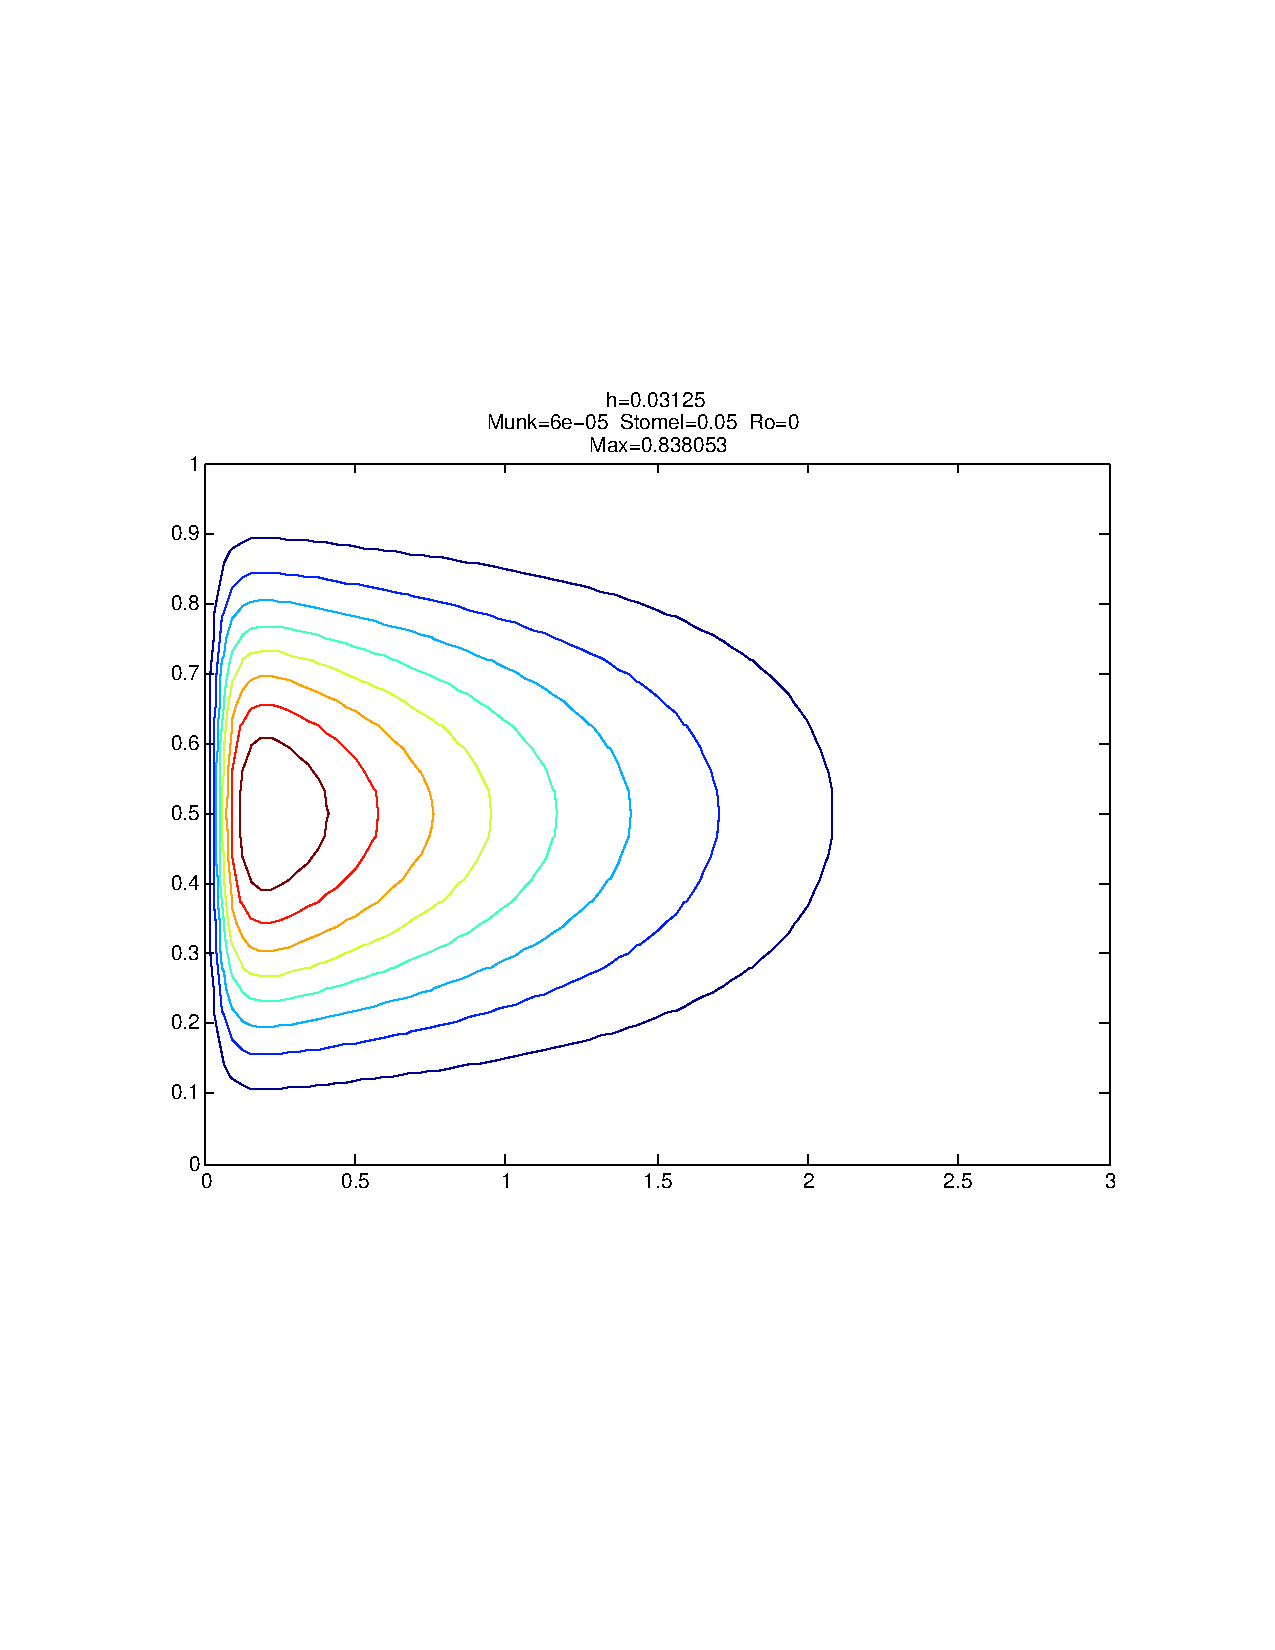
\includegraphics[trim=0 200 20 220, clip=true, scale=0.5]{StommelMunk2.pdf}
    \caption{Linear Stommel-Munk Model \eqref{eqn:SMProb}, Test 4 \cite{Cascon}: Streamlines of the approximation,
    $\psi^h$, $h=\frac{1}{32}$, and $28550$ DoFs.}
    \label{fig:SMe}
  \end{center}
\end{figure}

We note that the errors in \autoref{tab:SMeErrors} follow the theoretical rates
of convergence predicted by the estimates \eqref{eqn:H2Error} -
\eqref{eqn:L2Error} in \autoref{thm:Errors}. Again, we see that the orders of
convergence in \autoref{tab:SMeErrors} are close to the theoretical ones for the
fine meshes, but not as close for the coarse meshes. As stated previously, we
attribute this to the inaccuracies at the thin boundary layer on the left-hand
side (i.e., at $x=0$). The finer the mesh gets, the better this boundary layer
is captured and the better the numerical accuracy becomes.

\subsection{Stationary Quasigeostrophic Equations}\label{sse:SQGE}
This subsection presents results for the FE discretization of the streamfunction formulation of the
SQGE \eqref{sqge_psi_1} by using the Argyris element. Our computational domain is
$\Omega=[0,3]\times[0,1]$, the Reynolds number is $Re=1.667$, and the Rossby number is $Ro=10^{-4}$.
For completeness, we present results for two numerical tests, denoted by Test 5 and Test 6, both
corresponding to the exact solutions given in Test 1 and Test 2 of \cite{Cascon}, respectively.

\tbf{Test 5:}
In this test, we take the same exact solution presented in \emph{Test 3}, i.e.
\begin{equation}
  \psi(x,y) = \sin^2 \frac{\pi x}{3} \cdot \sin^2 \pi y.
  \label{eqn:StreamfunctionExact1}
\end{equation}
Again, the forcing term $F$ and homogeneous boundary conditions, $\psi = \frac{\partial
\psi}{\partial \mathbf{n}} = 0$, correspond to the exact solution \eqref{eqn:StreamfunctionExact1}.

\autoref{fig:SQGEsin} presents the streamlines of the approximate solution obtained by using the
Argyris Finite Element on a mesh with $h=\frac{1}{32}$ and $28550$ DoFs. We note that the
streamlines look as we expect and are similar to those given by Figure $7$ in \cite{Myers}, which
uses the same exact solution.  Since the exact solution is available, we can compute the errors in
various norms. \autoref{tab:SQGEsinErrors} presents the errors $e_0,\, e_1, \text{ and } e_2$ (i.e.,
the $L^2,\, H^1, \text{ and } H^2$ errors, respectively) for various values of the mesh sizes, $h$.

\begin{table}%[H]
\begin{center}
%{\scriptsize
\begin{tabular}{|c|c|c|c|c|c|c|c|}%c|c|}
  \hline
  $h$ & $DoFs$ & $e_0$ & $L_2$ order & $e_1$ & $H^1$ order & $e_2$ & $H^2$ order \\[0.2em] % & $e_{\infty}$ & $L_{\infty}$ order \\
  \hline
  $\nicefrac{1}{2}$ & $170$ & $0.005709$ & $-$ & $0.06033$ & $-$ & $1.087$ & $-$ \\[0.2em] % & $0.007512$ & $-$ \\
  $\nicefrac{1}{4}$ & $550$ & $3.726\times 10^{-5}$ & $7.259$ & $0.001086$ & $5.796$ & $0.04113$ & $4.724$ \\[0.2em] % & $2.828\times 10^{-5}$ & $8.053$ \\
  $\nicefrac{1}{8}$ & $1958$ & $3.597\times 10^{-7}$ & $6.695$ & $2.534\times 10^{-5}$ & $5.421$ & $0.002252$ & $4.191$ \\[0.2em] % & $3.488\times 10^{-7}$ & $6.341$ \\
  $\nicefrac{1}{16}$ & $7366$ & $4.648\times 10^{-9}$ & $6.274$ & $7.065\times 10^{-7}$ & $5.165$ & $0.0001344$ & $4.067$\\[0.2em] % & $4.696\times 10^{-9}$ & $6.215$ \\
  $\nicefrac{1}{32}$ & $28550$ & $6.737\times 10^{-11}$ & $6.108$ & $2.116\times 10^{-8}$ & $5.061$ & $8.26\times 10^{-6}$ & $4.024$ \\[0.2em] % & $6.965\times 10^{-11}$ & $6.075$ \\
 \hline
\end{tabular}
%}
\end{center}
\caption{Errors and Rate of Convergence for the Full SQGE \eqref{sqge_psi_1}, Test 5}
\label{tab:SQGEsinErrors}
\end{table}

\begin{figure}%[H]
  \begin{center}
    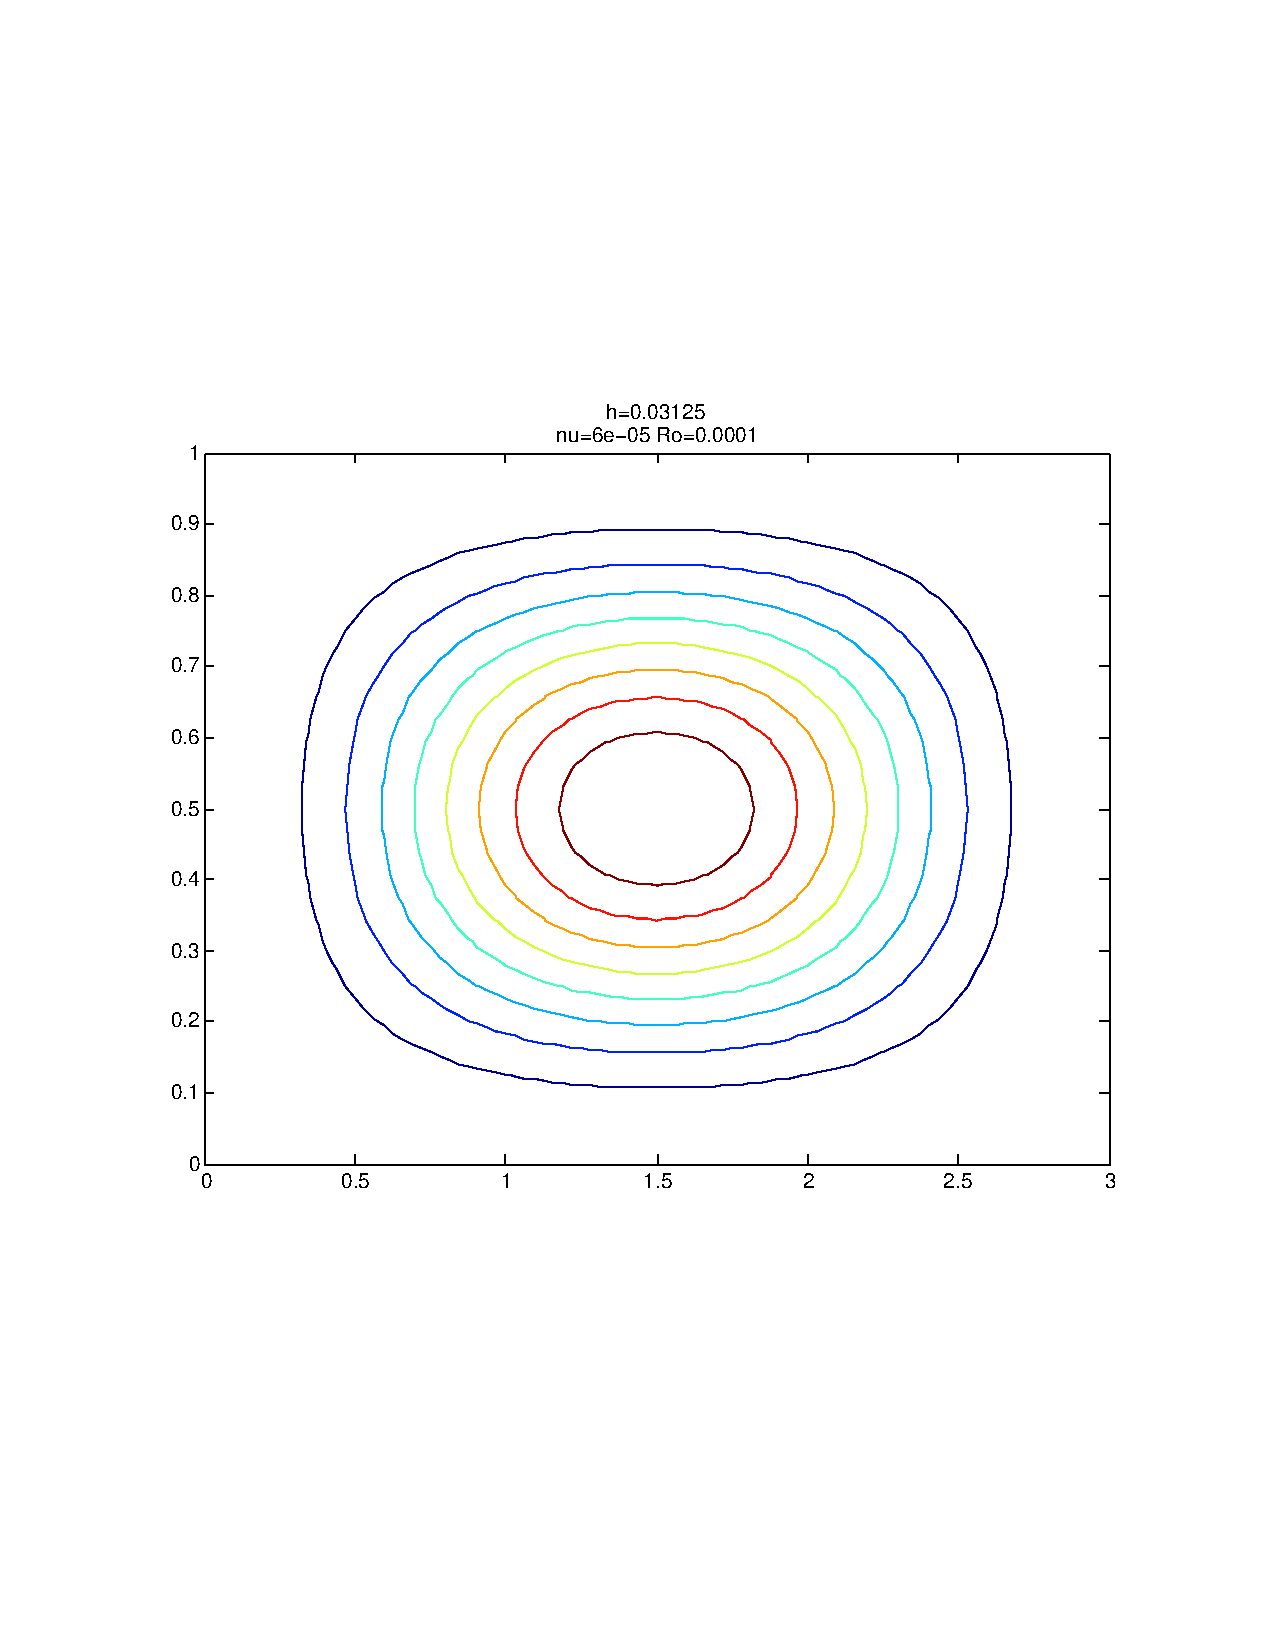
\includegraphics[trim=0 200 20 215, clip=true, scale=0.5]{SQGEsin.pdf}
    \label{fig:SQGEsin}
    \caption{Full SQGE \eqref{sqge_psi_1}, Test 5: Streamlines of the approximation,
    $\psi^h$, $h=\frac{1}{32}$, and $28550$ DoFs.}
  \end{center}
\end{figure}

We note that the errors in \autoref{tab:SQGEsinErrors} follow the theoretical rates of convergence
predicted by the estimates \eqref{eqn:H2Error} - \eqref{eqn:L2Error} in \autoref{thm:Errors}. Again,
since the exact solution \eqref{eqn:StreamfunctionExact1} does not display any boundary layers, we
see that the orders of convergence in \autoref{tab:SQGEsinErrors} are close to the theoretical ones for the fine meshes, but are higher
than expected for the for the coarse meshes.

\tbf{Test 6:}
In this test, we take the same exact solution as used in \emph{Test 4}, i.e.
\begin{equation}
  \psi(x,y) = \left[\left(1 - \frac{x}{3}\right)\left(1-e^{-20x}\right) \sin \pi y\right]^2.
  \label{eqn:StreamfunctionExact2}
\end{equation}
The forcing term $F$ and the homogeneous boundary conditions correspond to the exact solution
\eqref{eqn:StreamfunctionExact2}.

\autoref{fig:SQGEe} presents the streamlines of the approximate solution obtained by using the
Argyris Finite Element on a mesh with $h=\frac{1}{32}$ and $28550$ DoFs. We note that the
streamlines look as we expect and are similar to those given by Figure $10$ in \cite{Myers}, which
uses the same exact solution. Since the exact solution is available, we can compute the errors in
various norms. \autoref{tab:SQGEeErrors} presents the errors $e_0,\, e_1, \text{ and } e_2$ (i.e.,
the $L^2,\, H^1, \text{ and } H^2$ errors, respectively) for various values of the mesh sizes, $h$.

\begin{table}%[H]
\begin{center}
%{\small
\begin{tabular}{|c|c|c|c|c|c|c|c|}%c|c|}
  \hline
  $h$ & $DoFs$ & $e_0$ & $L_2$ order & $e_1$ & $H^1$ order & $e_2$ & $H^2$ order \\[0.2em] % & $e_{\infty}$ & $L_{\infty}$ order \\
  \hline
  $\nicefrac{1}{2}$ & $170$ & $0.3497$ & $-$ & $1.9$ & $-$ & $44.05$ & $-$ \\[0.2em] % & $0.353$ & $-$ \\
  $\nicefrac{1}{4}$ & $550$ & $0.0302$ & $3.533$ & $0.4279$ & $2.15$ & $21.74$ & $1.019$ \\[0.2em] % & $0.03188$ & $3.469$ \\
  $\nicefrac{1}{8}$ & $1958$ & $0.001507$ & $4.324$ & $0.06085$ & $2.814$ & $5.661$ & $1.941$ \\[0.2em] % & $0.002121$ & $3.91$ \\
  $\nicefrac{1}{16}$ & $7366$ & $3.225\times 10^{-5}$ & $5.547$ & $0.004042$ & $3.912$ & $0.7379$ & $2.94$ \\[0.2em] % & $3.832\times 10^{-5}$ & $5.79$ \\
  $\nicefrac{1}{32}$ & $28550$ & $5.672\times 10^{-7}$ & $5.829$ & $0.000161$ & $4.65$ & $0.0597$ & $3.628$ \\[0.2em] % & $8.91\times 10^{-7}$ & $5.426$ \\
 \hline
\end{tabular}
%}
\end{center}
\caption{Errors and Rate of Convergence for the Full SQGE \eqref{sqge_psi_1}, Test 6}
\label{tab:SQGEeErrors}
\end{table}

\begin{figure}%[H]
  \begin{center}
    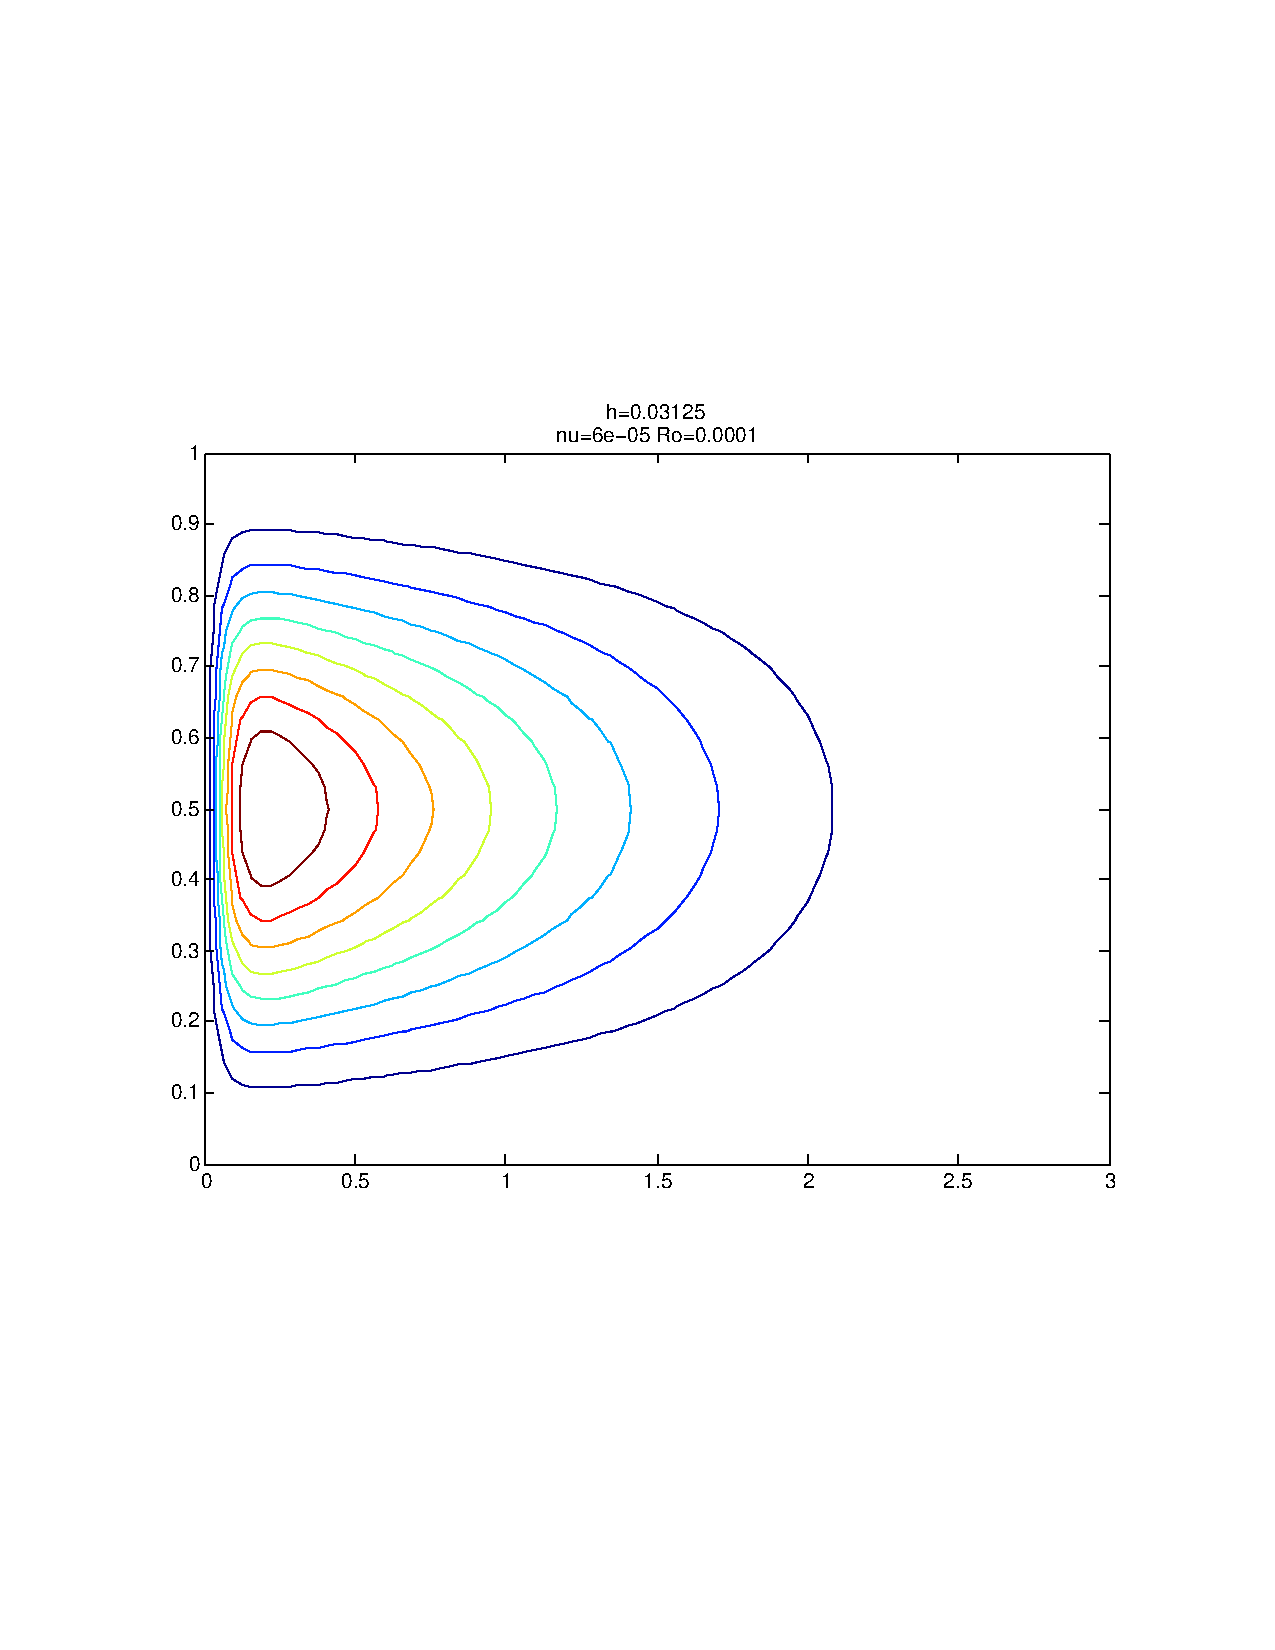
\includegraphics[trim=0 200 20 215, clip=true, scale=0.5]{SQGEe.pdf}
    \caption{Full SQGE \eqref{sqge_psi_1}, Test 6: Streamlines of the approximation,
    $\psi^h$, $h=\frac{1}{32}$, and $28550$ DoFs.}
    \label{fig:SQGEe}
  \end{center}
\end{figure}

We note that the errors in \autoref{tab:SQGEeErrors} follow the theoretical rates of convergence
predicted by the estimates \eqref{eqn:H2Error} - \eqref{eqn:L2Error} in \autoref{thm:Errors}. Again
for an exact solution which has a western boundary layer, we see that the orders of convergence in \autoref{tab:SQGEeErrors} are close to the theoretical ones for the fine meshes, but
not as close for the coarse meshes. We attribute this to the inaccuracies at the thin boundary layer
on the left-hand side (i.e., at $x=0$). The finer the mesh gets, the better this boundary layer is
captured and the better the numerical accuracy becomes.
